\chapter{Theory and Methods}
\begin{comment}

% Questa è la parte che avevo inizialmente scritto io
To investigate the optical jitter affecting a pulsed laser source, it is first essential to establish a clear and simple definition of what jitter is.
\autoref{Sec:Def-Jitter} is dedicated to this purpose, beginning with a basic definition derived from signal theory, zooming in into the topic and introducing some key definitions, as well as an initial example to then end up providing a proper categorization of the sources of jitter.

\autoref{sec:Def-Pulses} provides the reader with the essential background on optical pulses, including key temporal properties and their connection to the spectral domain, with the important mention of the Time-Bandwidth product.
Finally, \autoref{sec:Def-Techniques} offers the theoretical foundation behind the main experimental techniques used in this work, serving as a conceptual bridge between the theory and the measurements discussed in later chapters.



\section{Timing Jitter}
\label{Sec:Def-Jitter}

To better understand what jitter means in the context of optical pulses, we must first give the general definition.

Jitter was originally defined in signal theory as the deviation of the timing instants 
of a sequence of events from their ideal positions in time.
It can affect not only signals that are meant to be rhythmically constant—such as the ticks of a 
clock—but also repetitive or quasi-periodic signals that may include asynchronous events [IEEE Standard \cite{General_IEEE}].

In this thesis, we study jitter in the context of optical pulses, which serve as carriers of timing information
 for our experimental instruments and detectors. Given this focus, the more specific notion of timing jitter is most relevant.
According to the IEEE, timing jitter is defined as the deviation of 
the actual timing instants of a waveform from their ideal temporal positions \cite{General_IEEE}.

We introduce for a better understanding the \autoref{AddAmpl}, where it's shown the timing jitter caused by an additive amplitude noise on the timing signal.
In this image the noisy rising edge of the waveform crosses the detection threshold over a range of reference instants that deviate from the ideal reference position. Throughout this thesis this is the first time that we mention the role of thresholding, and it is not a case that this will happen already at the very beginning like here, especially because it is fundamental to understand that only one threshold crossing will be detected, per single part of the waveform. The only important question is when such event will happen, with respect of the ideal position in time. This is the whole idea behind the study of timing jitter.

\begin{figure}[hbtp]
\centering
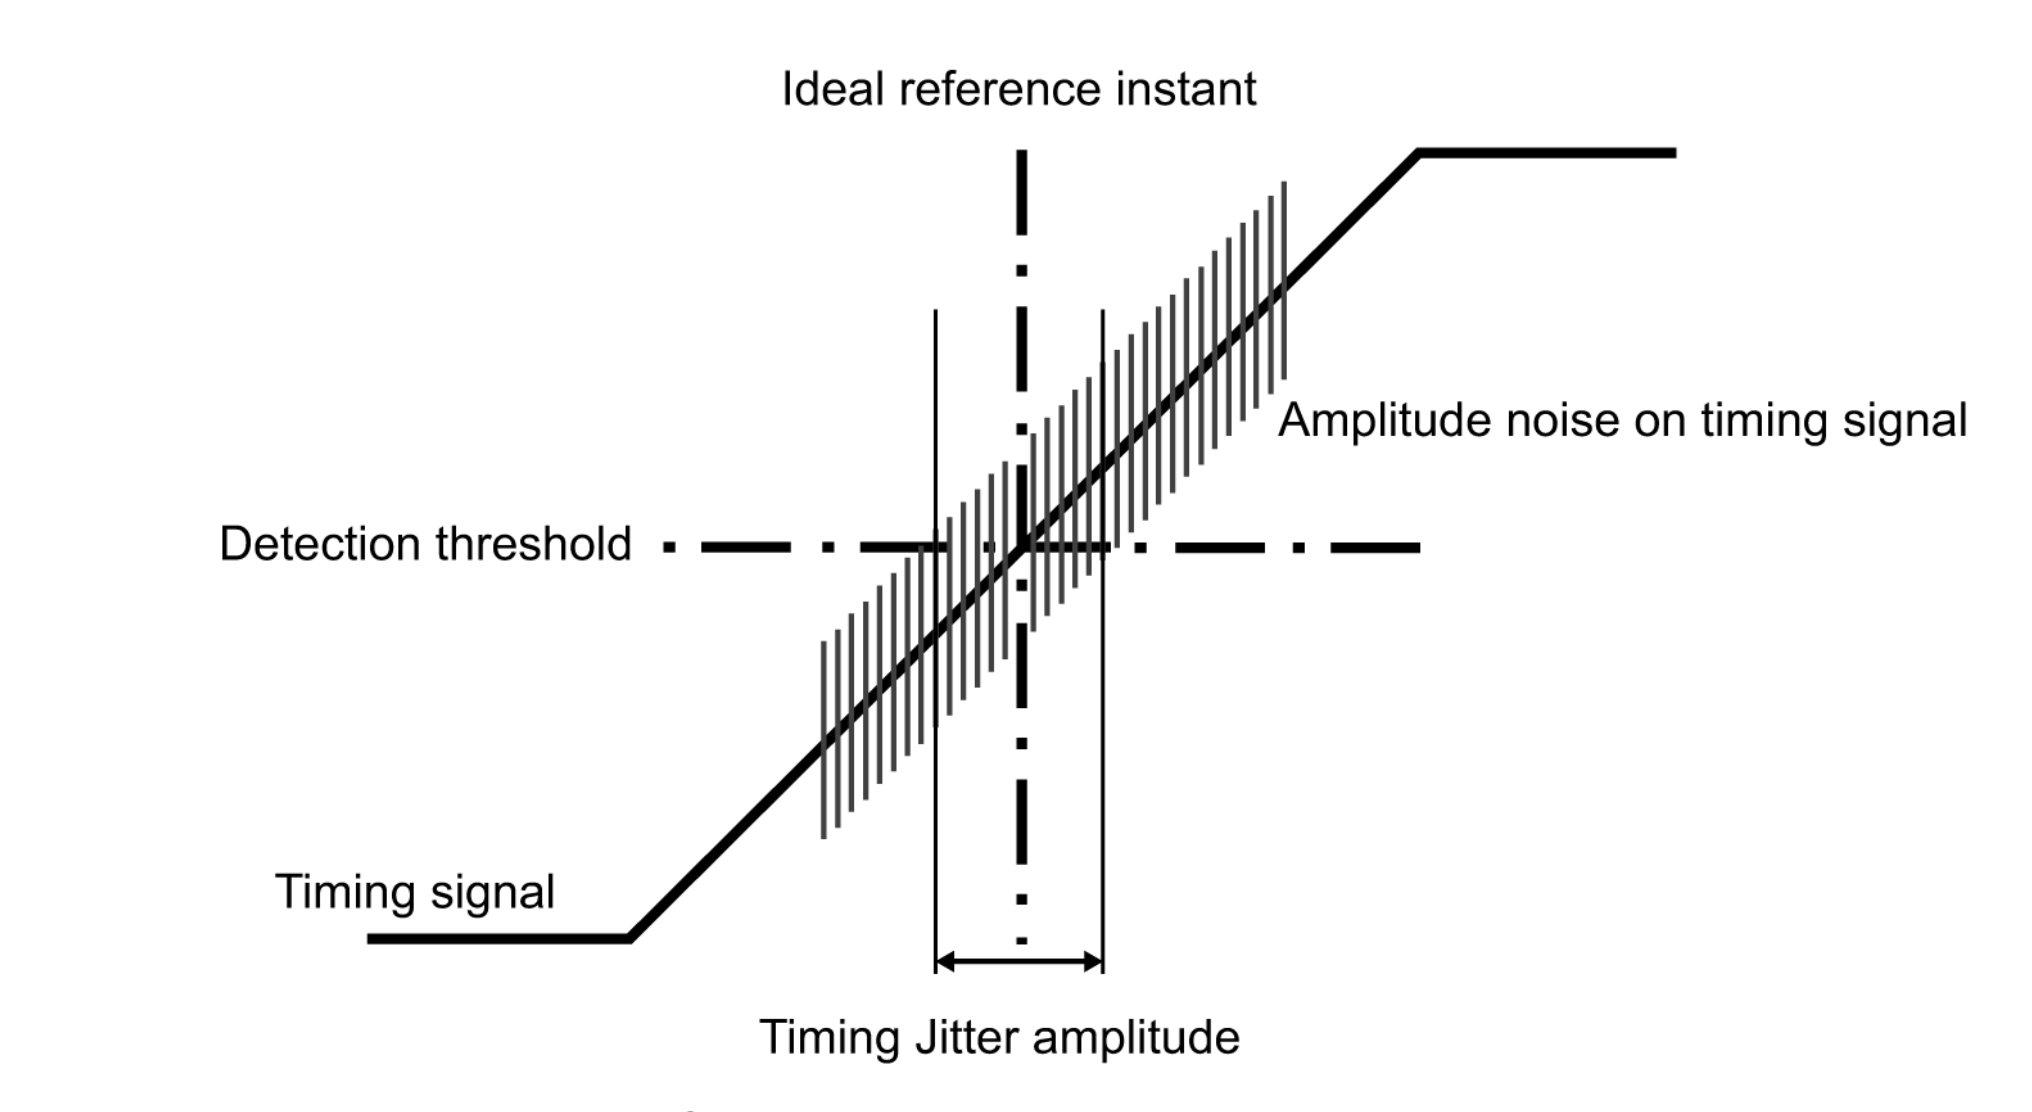
\includegraphics[width=1\textwidth]{AmplitudeAdditiveNoise}
\caption{ Example of timing Jitter induced by an additive amplitude noise \cite{General_IEEE}}
 \label{AddAmpl}
\end{figure} 


\end{comment}

%Questa è la versione ottimizzata una prima volta
To investigate the optical jitter affecting a pulsed laser source, it is first essential to establish a clear and simple definition of what jitter is.  
\autoref{Sec:Def-Jitter} is dedicated to this purpose, beginning with a fundamental definition derived from signal theory, then gradually refining the concept with key terminology and a relevant example. The section concludes by introducing a basic categorization of the main jitter sources.

\autoref{sec:Def-Pulses} provides the reader with the essential background on optical pulses, highlighting their temporal properties and their connection to the spectral domain. Particular attention is given to the Time-Bandwidth product, which plays a central role in later analysis.

Finally, \autoref{sec:Def-Techniques} outlines the theoretical background of the experimental techniques employed throughout this work, serving as a conceptual bridge between the physical principles and the measurements presented in the following chapters.

\section{Timing Jitter}
\label{Sec:Def-Jitter}

To understand jitter in the context of optical pulses, we must begin with its general definition.

Jitter was originally introduced in signal theory as the deviation of the timing instants of a sequence of events from their ideal temporal positions. It can affect not only signals designed to be rhythmically constant—such as clock ticks—but also repetitive or quasi-periodic signals, including those with asynchronous components~\cite{General_IEEE}.

In this thesis, we focus on jitter as it appears in optical pulses, which serve as carriers of precise timing information for our instruments and detectors. For this reason, the specific notion of \emph{timing jitter} is most relevant. According to the IEEE, timing jitter is defined as the deviation of the actual timing instants of a waveform from their ideal temporal positions~\cite{General_IEEE}.

\autoref{AddAmpl} shows an example of timing jitter induced by additive amplitude noise on a signal’s rising edge. In the figure, the noisy waveform crosses the detection threshold over a spread of time instants, deviating from the ideal reference point.



\begin{figure}[hbtp]
\centering
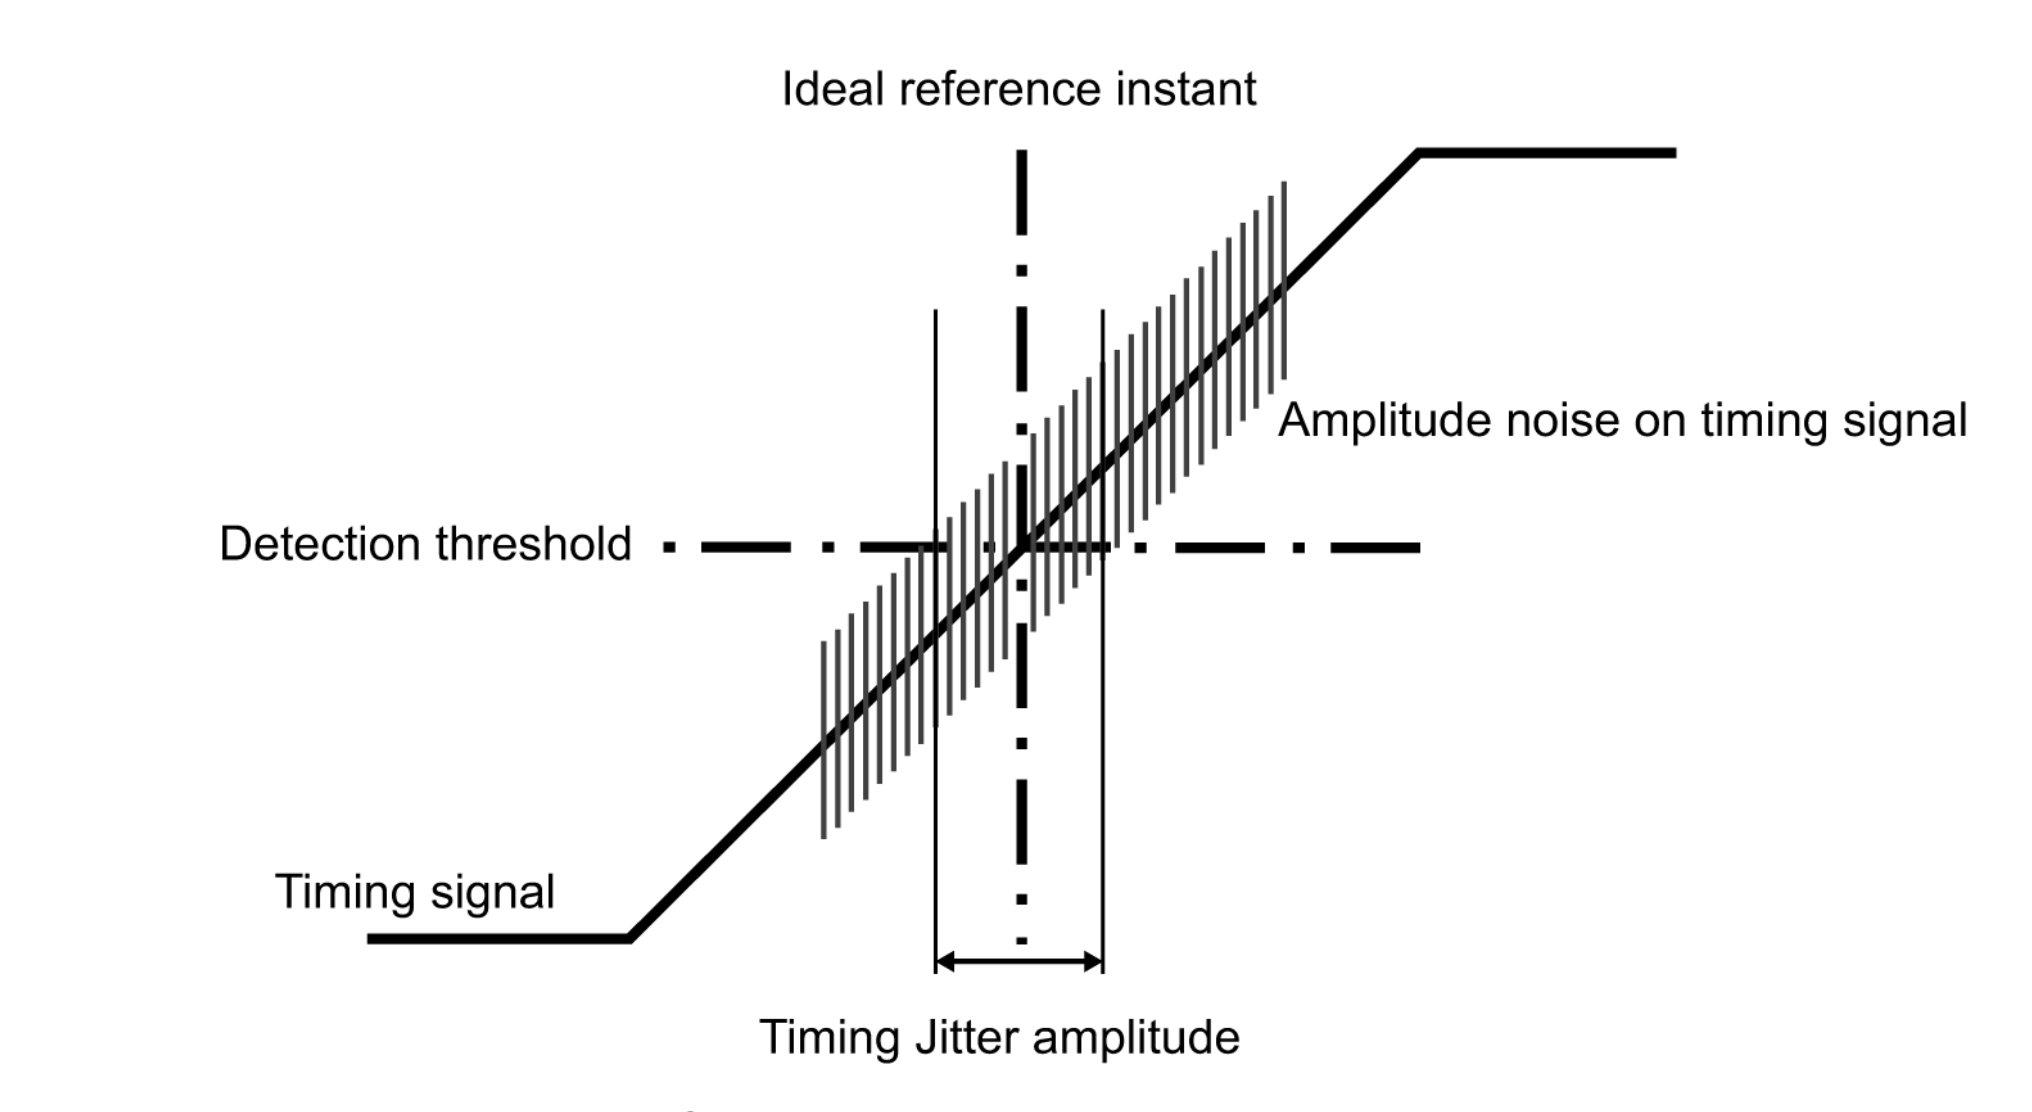
\includegraphics[width=1\textwidth]{AmplitudeAdditiveNoise}
\caption{Example of timing jitter induced by additive amplitude noise~\cite{General_IEEE}.}
\label{AddAmpl}
\end{figure}

%INIZIO DEL SOTTOCAPITOLO CON LA DESCRIZIONE DELLA CATEGORIZZAZIONE DEL TIMING JITTER IN RANDOMICO O DETERMINISTICO
\subsection{Classification of timing jitter sources}

Timing jitter can be broadly classified into two main categories: \emph{deterministic jitter (DJ)} and \emph{random jitter (RJ)}. 

%Deterministic jitter arises from predictable, repeatable sources such as crosstalk, power supply noise, or duty cycle distortion. In contrast, random jitter originates from stochastic processes, such as thermal noise or quantum fluctuations in detection, and is inherently unbounded over long timescales.

We identify with the name Random jitter (RJ) all those jitter sources that don't allow successive references to be systematically determined, and this is the reason why a statistical treatment is needed.
By applying the Central limit theory, RJ can be treated as a mean zero distortion of the waveform, with an unbounded underlying gaussian probability density function $f_{RJ}(x)$.

\begin{equation}
f_{RJ}(x) = \frac{1}{\sigma \sqrt{2 \pi }}e^{-\frac{x^2}{2 \sigma ^2}}
\label{eq:RandJitter}
\end{equation}
In this function we can identify x as the random variable that eventually gives contribution to the Total Jitter (TJ), as well as the standard deviation $\sigma$ that defines entirely the features of $f_{RJ}(x)$.

Random Jitter is studied usually together with a large number of timing errors detected, because with the assumption of low contributions in terms of DJ, we can understand the features of the underlying probability density function.


%In presence of low contributions in terms of deterministic jitter, Random Jitter can be studied starting from a considerable number of timing errors observed, to which it's possible to draw a statistic and proceed with the analysis.

\autoref{RandomIMG} (a) shows how the pdf $f_{RJ}(x)$ describes the random contribution in terms of jitter to the actual position of the waveform. %without forgetting that such random extraction  happens for every rising or falling edge of the waveform independently.

When the position of a reference event on the waveform can be deterministically retrieved from the previous few ones, we are dealing with deterministic jitter. While DJ has usually several sources, it is common practice to decompose it within the different types of behavior.
The key difference with RJ lies in the replicable trait of its contributions, in the scenario in which we have fully understood every jitter source.
By being Systemic, DJ doesn't limits to a constant type of behavior, but instead gives an explanation to periodic and non periodic bounded patterns \cite{General_IEEE}. 
\autoref{RandomIMG} (b) shows how the presence of a deterministic external aggressor signal striking the input waveform, causes a shift in the actual detection of the threshold crossing. To a greater extent, we can safely say that such behavior happens also in the scenario of several sources acting together in a deterministic way as presented also in \cite{Crosstalk_IEEE1}.

%The modelization of the DJ sources, finds its foundations in an alternative use of PDFs, that differs from the ones that we encountered before for the RJ, in terms of domain being always bounded.

Despite the deterministic nature of these sources, the mathematical treatment doesn't differ extremely from the one seen for the RJ, with the key difference being the domain of definition, that results here strictly bounded. As per the last published article about timing jitter belonging to the IEEE, the main sources of DJ can be divided onto Data-dependent Jitter(DDJ), Periodic Jitter (PJ) and Bounded Uncorrelated Jitter(BUJ).

Usually at the first level of any jitter-related study there is the measure of the amount of Total Jitter (TJ), that includes both deterministic and random contributions. Since both of these are described by PDFs, the resulting total jitter happens to be the linear convolution of the Random and Deterministic complessive density functions.
While in principle the $f_{RJ}(x)$ is a Gaussian, the other argument of the convolition happens to be the convolution itself of every deterministic source. 

\begin{equation}
f_{DJ}(x) = f_{DDJ}(x) \circledast f_{PJ}(x) \circledast f_{BUJ}(x) 
\label{eq:DetJitterConvo}
\end{equation}

\begin{equation}
f_{TJ}(x) = f_{DJ}(x) \circledast f_{RJ}(x) 
\label{eq:TOTjitterConvo}
\end{equation}




\begin{figure}[hbtp]
\centering
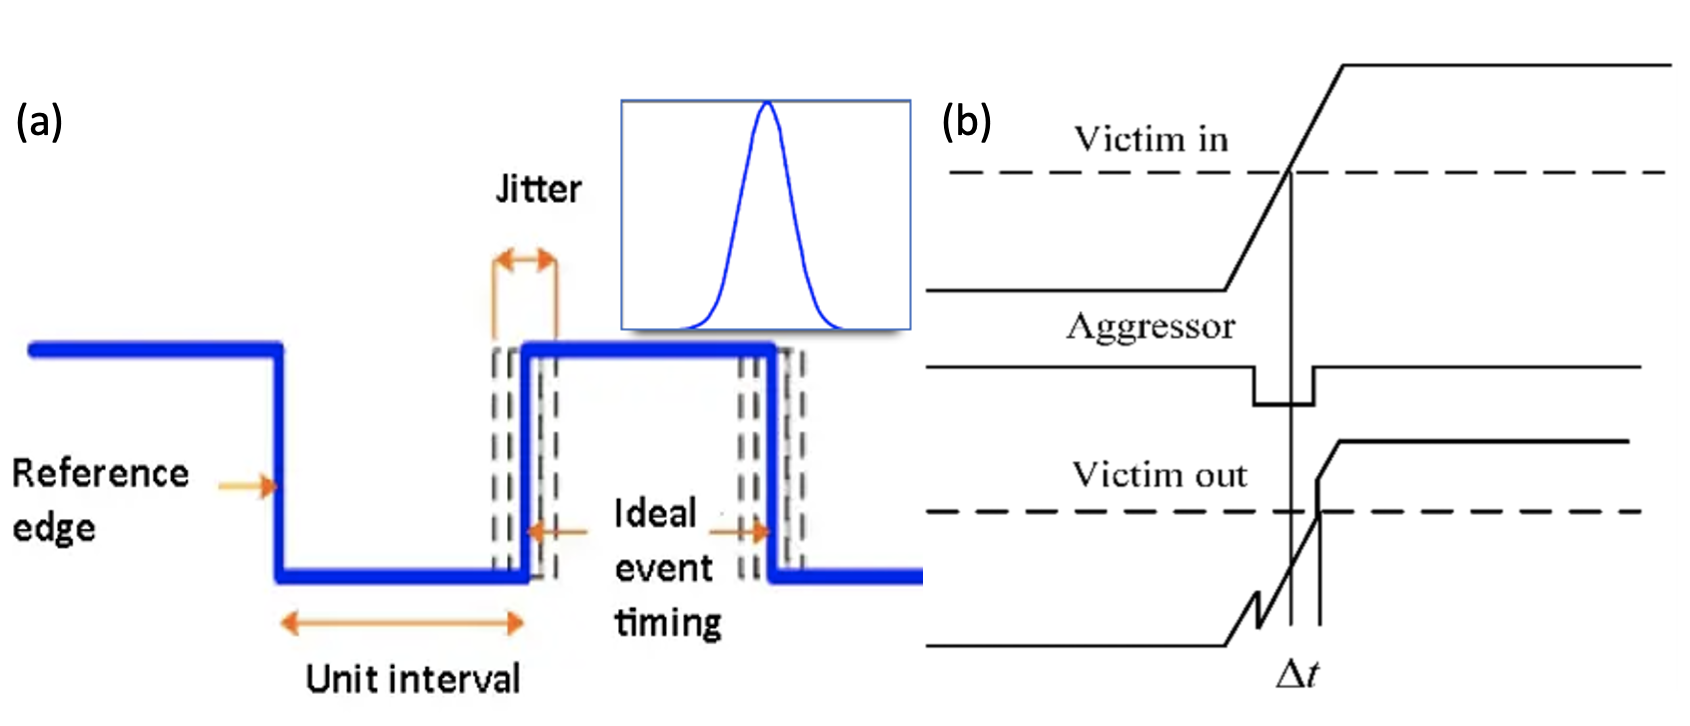
\includegraphics[width=1\textwidth]{RandomCrosstalk}
\caption{(a)Visual representation of the concept of stochastic contribution to timing jitter caused by RJ, here represented with its relative pdf.
(b) Sketch representing the timing jitter caused by an external crosstalk aggressor signal, striking the reference signal and causing the detection event to shift in time because of that.}
\label{RandomIMG}
\end{figure}


\section{Optical pulses}
\label{sec:Def-Pulses}
%Scaletta di cose da dire secondo il nostro caro amico in comune !!!
\begin{comment}
1. Introduction to Optical Pulses
Define what an optical pulse is (brief burst of electromagnetic energy in the optical domain).
Mention the typical time scales involved (fs–ns), depending on the source.
Relate it to your experiment: pulsed laser sources as timing references.
2. Key Temporal Properties
Pulse duration (FWHM): define it and note that it's a crucial timing parameter.
Amplitude and energy: mention intensity profiles, peak power vs. average power.
Repetition rate / period: introduce the temporal spacing between pulses in a mode-locked laser.
3. Temporal and Spectral Domain
Discuss the duality: every pulse has a spectral counterpart.
Present the Fourier transform relationship (not too mathematically, unless your audience expects it).
Emphasize that shorter pulses have broader spectra.
Show how the pulse shape (Gaussian, sech², Lorentzian) affects both time and frequency profiles.
4. Pulse Evolution and Distortion
Briefly describe how optical pulses evolve when propagating through media (e.g., fibers).
Introduce group velocity dispersion (GVD) as the main reason for pulse broadening.
Mention nonlinear effects only if relevant later in your thesis (e.g., self-phase modulation).
5. Time-Bandwidth Product
Define the TBP and explain its role as a measure of pulse quality.
Include TBP values for common shapes: Gaussian (0.44), sech² (0.315), etc.
Explain that TBP sets a fundamental limit: bandwidth and pulse duration cannot both be arbitrarily small.
Optionally, relate to your experiment: estimating the expected pulse duration from spectral width.


Citazioni da utilizzare :
per la parte della definizione delle prime definizioni e delle formule che collegano le stesse alle cose successive procedi con l'utilizzo di questa
\cite{shapiro1984, Paschotta_2007_light_pulses}
\end{comment}
Throughout this thesis we worked with pulsed laser sources, whose essential feature is the optical pulse.
Lasers can operate essentially in two completely organized regimes : the continuous wavelength lasing (CW) or the mode-locked pulsing.
When the set of longitudinal modes in the laser cavity is maintained in fixed phase and amplitude conditions the output laser beam will be a well defined function of time, realizing a mode-locked pulse train \cite{shapiro1984}.

\subsection{Repetition rate and Pulse duration}
Among the basic properties of optical pulses, the repetition rate $f_{\text{rep}}$ and the optical pulse duration are two key parameters that should be mentioned before any mathematical derivation.

The pulse repetition rate, sometimes also called pulse repetition frequency, of a pulsed laser source is defined as the number of emitted pulses in a second, or alternatively the inverse temporal pulse spacing \cite{RP2005_rep_rate}.

The temporal duration, also referred as pulse width, of an optical pulse finds its foundations in the concept of Full Width Half-Magnitude (FWHM). While this definition is widely accepted, for some specific cases (e.g. solitons described by a $sech^2$ function) it is preferred the use of a duration parameter $\tau$ that is approximately the ratio between the FWHM and a conversion parameter valued 1.726 \cite{RP2005_duration}. 

\subsection{Mathematical derivation of the temporal and spectral intensity functions}
In order to define even more the features of the optical pulses we should first define a pair of Fourier integrals :
\begin{equation}
E(t) = \frac{1}{\sqrt{2\pi}}\int_{-\infty}^{+\infty} e(\omega)e^{-i\omega t}\, d\omega
\label{eq:ElectricalField}
\end{equation}

\begin{equation}
e(\omega) = \frac{1}{\sqrt{2\pi}}\int_{-\infty}^{+\infty} E(t)e^{i\omega t}\, dt
\label{eq:FT_Electrical}
\end{equation}

We then define the complex signal $V(t)$ of a plane wave optical pulse, related to the magitude of the electrical field $E(t)$ described in \autoref{eq:ElectricalField} at a fixed point in the space writing the following equations :

\begin{equation}
V(t) = \frac{1}{\sqrt{2\pi}}\int_{0}^{+\infty} 2e(\omega)e^{-i\omega t}\, d\omega
= \frac{1}{\sqrt{2\pi}}\int_{0}^{+\infty} \nu(\omega)e^{-i\omega t}\, d\omega
\label{eq:OptPulse1}
\end{equation}

To achieve the final formulation of \autoref{eq:OptPulse1} the amplitudes of the negative frequency components of \autoref{eq:ElectricalField} are suppressed, while the positive ones are instead doubled.
It follows that 

\begin{align}
\nu(\omega) &= \frac{1}{\sqrt{2\pi}}\int_{-\infty}^{+\infty} V(t)e^{+i\omega t}\, dt \notag \\
            &= 2e(\omega) \quad \quad (\omega > 0) \notag \\
            &= 0  \quad \quad \quad (\omega < 0)
\label{eq:OptPulseFreq}
\end{align}

These complex functions, namely $V(t)$ as well as $\nu (t)$ are perfect candidates to define the optical pulse in the time and in the frequency domain repectively.

Moreover this formulation helps defining the spectral amplitude and the spectral phase associated to the frequency domain formulation.
In particular, by writing

\begin{equation}
\nu (\omega) = a(\omega) e^{-i\phi (\omega)}
\label{eq:SpecFeatures}
\end{equation}

we will recognize $a(\omega)$ as the spectral amplitude and $\phi (\omega)$ as the spectral phase \cite{Bradley1974}.
When the pulse bandwidth $\Delta \omega$ is narrow compared to the mean optical frequency $\omega _0$ we can then write 

\begin{equation}
    V(t)=A(t)e^{i(\Phi (t)-\omega _{0} t )}
\label{eq:OptSynthetic}
\end{equation}

In the case of study of optical pulses, the temporal amplitude $A(t)$ and the temporal phase $\Phi (t)$ of the optical frequency wave are both slowly varying functions in the time domain. Thus the instantaneous intensity associated to the optical pulse is 

\begin{align}
    I(t) &= V(t)V^{*}(t) \notag \\
         &= A^{2}(t)
\label{eq:OptIntensity}
\end{align}

Following the same steps as in the previous case it is also possible to define the spectral intensity function
\begin{align}
    i(\omega) &= \nu (\omega)\nu ^{*}(\omega) \notag \\
              &= a^2 (\omega)
\label{eq:OptFreqIntensity}
\end{align}

\subsection{The Time-Bandwidth product}
According to the Parceval's Theorem the total energy of a pulse is proportional to the area under either of the spectral or intensity profiles.
\begin{equation}
    \int_{-\infty}^{+\infty} I(t)\, dt \quad \quad  \int_{0}^{+\infty} i(\omega)\, d\omega
\label{eq:AreaIntensities}
\end{equation}

This notation clearly enhances the symmetry between the temporal and frequancy descriptions of the pulse.
Regardless of the description that we wish to present, the optical pulse is completely defined by a phase and an intensity. From the mathematical perspective there is a one-on-one corrispondence between the two different formulation of the intensity profile.

More specifically the general property that regulates the mutual mapping that links the two formulations arises from the Uncertainty Principle, stating that : 
\begin{equation}
    \frac{(\Delta \omega \Delta t)}{2\pi} \ge K
\label{eq:Uncertainty}
\end{equation}
Where K is by constant value whose value depends on the shapes of the two intensity profiles.

Usually in the context of pulsed laser source, pulses can be described as "Transform-limited" or also "bandwidth-limited" : this only happens when given a certain bandwidth in the temporal domain it is produced the shortest possible pulse obtainable.
In such a case the actual duration is 
\begin{equation}
    \Delta t = \frac{2\pi K}{\Delta \omega}
\label{eq:TransLimited}
\end{equation}

In the scientific literature the value of $(\Delta \omega \Delta t)/2\pi$ is referred as "time-bandwidth product" $P$ and represent a key parameter in the field of ultra short laser pulses. On behalf of the solitons created by mode locked lasers, the value of P is a good indicator to assess the extent to which the production of ideal pulses is being achieved \cite{shapiro1984}.
%Finally, optical pulses that are completely devoid of amplitude or frequency are defined "bandwidth-limited".

Let us introduce a basic example to conclude the treatment: The gaussian-shaped spectral intensity profile.
\begin{equation}
    i(\omega) = e^{\frac{-(\omega - \omega _0 )^2)}{\alpha}}
\label{eq:exampleSpectral}
\end{equation}

In this scenario also in the temporal domain the intensity has the shape of a gaussian 
\begin{equation}
    I(t)=\alpha e^{-\alpha (t-t_0)^2}
\label{eq:exampleTemporal}
\end{equation}

In this ideal scenario, the constant parameter $K$, introduced before in \autoref{eq:Uncertainty}, will result in being $K = (2ln2)/\pi = 0.441$.


\section{HBT and TCSPC: Measuring and interpreting ps optical jitter}
\label{sec:Def-Techniques}
\begin{comment}
Scaletta di cose da dire secondo il nostro caro amico in comune !!!

 ====================== INIZIO SCALETTA SEZIONE TECNICHE SPERIMENTALI ======================
 1. The Hanbury Brown Twiss effect and the second-order correlation function
    - Introdurre g^{(2)}(τ) come misura statistica delle correlazioni temporali tra eventi di rivelazione fotonica.
    - Spiegare il significato per diverse sorgenti luminose: luce classica, termica, coerente, singoli fotoni.
    - Esplicitare la sua forma normalizzata:
        g^{(2)}(τ) = ⟨I(t) I(t+τ)⟩ / ⟨I(t)⟩^2
      oppure per rivelazione discreta:
              g^{(2)}(τ) ∝ N_{12}(τ) / (N_1 ⋅ N_2)
                 - Interpretazione qualitativa:
       • g^{(2)}(0) < 1 → luce sub-poissoniana (quantistica, antibunching)
        • g^{(2)}(0) = 1 → luce coerente (Poissoniana)
        • g^{(2)}(0) > 1 → luce termica (bunched)

 2. Configurazione HBT
    - Descrivere lo schema con beam splitter: un impulso ottico diviso su due rivelatori.
    - Obiettivo: misurare conteggi in coincidenza tra rivelatori.
    - Evidenziare l'importanza dei ritardi temporali tra eventi.
    - Limitazioni:
        • Risoluzione temporale limitata dalla risposta dei rivelatori e dell'elettronica.
        • Necessaria normalizzazione accurata.

 3. TCSPC (Time-Correlated Single Photon Counting)
    - Principio: registrare intervallo temporale tra un trigger (es. sync laser) e rivelazione di un singolo fotone.
    - Si accumula un istogramma su molti impulsi.
    - Risultato: profilo temporale della probabilità di rivelazione (convoluto con risposta del sistema).
    - Perché è così preciso: sensibilità a singolo fotone, risoluzione su scala dei ps.
    - Limitazioni: pile-up, tempo morto del rivelatore.

 4. Ruolo nel contesto della tesi
    - Confronto tra TCSPC e HBT
        • TCSPC usato per analizzare jitter temporale e forma degli impulsi.
        • HBT usato per costruire g^{(2)}(τ) e studiare correlazioni temporali.
    - Entrambe le tecniche sensibili al jitter temporale dei rivelatori.
    - Entrambe contribuiscono a caratterizzare la risposta temporale complessiva del sistema.
 ====================== FINE SCALETTA ======================
\end{comment}

% Inizio della parte scritta di questo capitolo : mi baso su quello che mi ha consigliato Ugo di dire qui in fase di esordio
%The state of the art of modern single photon detector has managed to reach time resolutions easily higher than conventional high-speed photo diodes
The state of the art of modern single photon detectors have easily surpassed the time resolution of conventional high-speed photodiodes.

Although we study pulsed laser sources, and not single photon light, our analysis rely on a detection system based on a \emph{superconducting nanowire single photon detector (SNSPD)}.
%Throughout this thesis we study optical pulses using a \emph{superconducting nanowire single photon detector (SNSPD)}

\autoref{subs:HBT} presents the Hanbury Brown Twiss (HBT) experiment, as well as its tight binding with the second-order correlation function.
\autoref{subs:TCSPC} includes a description of the functioning principle of the time-correlated single photon counting (TCSPC) procedure, a key way to inspect the shape of the optical pulses with a probabilistic approach.
%In the end \autoref{subs:comparison} will finally give a comparison in terms of timing jitter to these two experimental techniques, providing the mathematical framework that lies behind the TSCPC and the HBT Start Stop, two sides of the same medal






\subsection{The HBT experiment and the second order correlation function}
\label{subs:HBT}
%The Hanbury Brown Twiss experiment is a reliable choice to minimize the strong behavior brought
Using an SNSPD requires to take into account key features like the timing jitter, the detection probability as well as the detector deadtime.
By definition the deadtime is the time required by the nanowire to recover from the last detection in order to be ready to receive the next one. 
The order of magnitude of this parameter is generally of nanoseconds : in this scenario a useful strategy is to split the incoming pulsed light into two different fibers, with the use of a 50:50 fiber directional coupler, to carry out detections with twice the amount of detectors.

This type of experimental setup belongs to the name of two english scientists, Hanbury Brown and Richard Twiss, who developed this intensity interferometer to study the size of Sirius in the mid 50s \cite{1956Natur.178.1046H}.

This experimental setup can be used either in a Start/Stop mode, collecting on an histogram the relative times measured between the \emph{START} and the \emph{STOP} consecutive detections of the two detectors, or otherwise by correlating the two streams of clicks. %Richiede manutenzione questa frase !!!!
In both these cases the final goal is the refinement of the second-order correlation function $g^{2}(\tau)$, with the key difference being that in the latter scenario the resulting coincidences histogram is not limited to consecutive detections like in the first, limited, case.

The $g^{2}(\tau)$ quantifies the intensity fluctuations in the correlated signal and the classical formulation is shown in \autoref{Classical_g2}.

\begin{equation}
g^{(2)}(\tau) = \frac{\langle I_2(t) I_3(t + \tau) \rangle}{\langle I_2(t) \rangle \langle I_3(t + \tau) \rangle}
\label{Classical_g2}
\end{equation}
In this equation $I(t)$ represent the intensity of the light at the time $t$, while the subscript indicates the detector, according to the visual representation  provided by \autoref{HBT_Sketch}.

A special focus in this thesis has been the refinement of the $g^{2}(\tau)$ from the two streams of detections belonging to the two detectors.
In this scenario the actual intensities measured at the time t are expressed by the number of counts in the specific temporal binsize, realizing 
%Aggiungi qui la successiva equazione, come da esempio !!




\begin{figure}[hbtp]
\centering
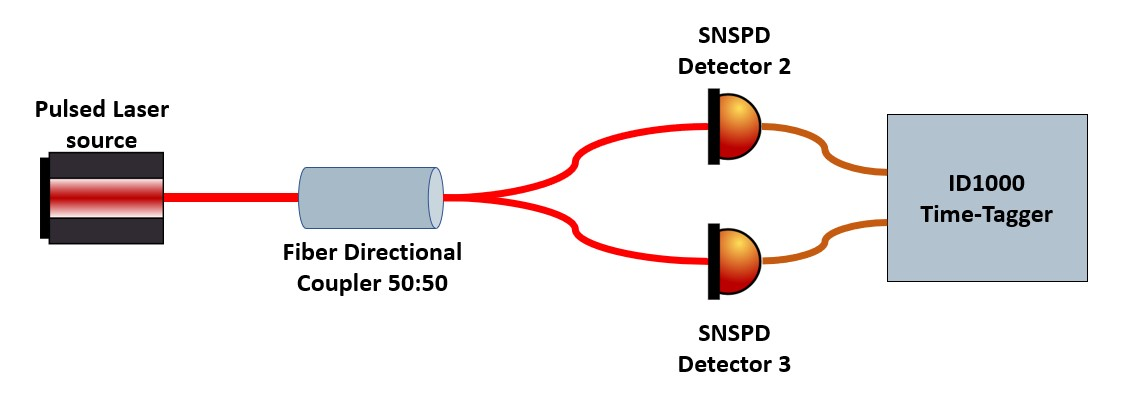
\includegraphics[width=1\textwidth]{HBT_Sketch}
\caption{Visual Representation of the Hanbury-Brown-Twiss setup implemented in the thesis}
\label{HBT_Sketch}
\end{figure}



\subsection{Time-correlated single photon counting}
\label{subs:TCSPC}
\begin{comment}
    Tutte le informazioni le trovi alla pagina (effettiva) 100 del libro TCSPC TOTAL, che ho messo nella cartella material di OneDrive
\end{comment}







\begin{figure}[hbtp]
\centering
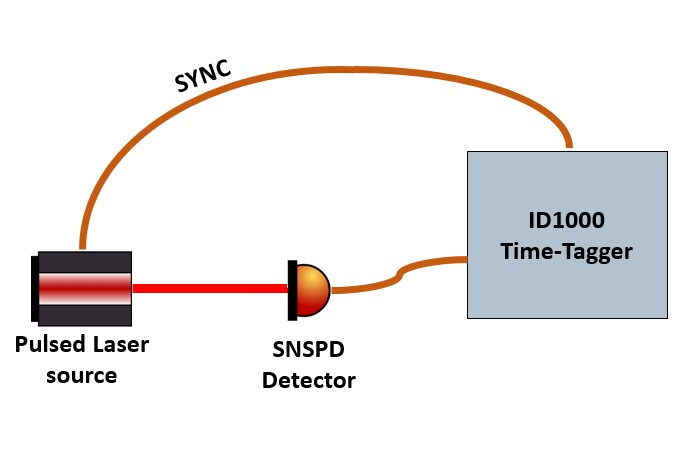
\includegraphics[width=0.75\textwidth]{TCSPC_sketch}
\caption{Visual Representation of the TCSPC setup implemented in the thesis}
\label{TCSPC_Sketch}
\end{figure}

\subsection{Second order correlation function}
\label{subs:comparison}
